%% LyX 2.2.4 created this file.  For more info, see http://www.lyx.org/.
%% Do not edit unless you really know what you are doing.
\documentclass[twoside]{bioinfo}
\setcounter{secnumdepth}{3}
\setcounter{tocdepth}{3}
\usepackage[active]{srcltx}
\usepackage{textcomp}
\usepackage{graphicx}

\makeatletter
%%%%%%%%%%%%%%%%%%%%%%%%%%%%%% User specified LaTeX commands.
\copyrightyear{2015} \pubyear{2015}

\access{Advance Access Publication Date: Day Month Year}
\appnotes{Manuscript Category}

\let\cite\citep

% Luis Garreta defs
\renewcommand{\textrightarrow}{$\rightarrow$}

\makeatother

\begin{document}
\firstpage{1}

\subtitle{Genetics and population analysis}

\title[short Title]{MultiGWAS: A tool for GWAS analysis on tetraploid organisms by integrating results of four GWAS software}

\author[Sample \textit{et~al}.]{Luis Garreta\,$^{\text{\sfb 1,}}$, Ivania Cer�n-Souza\,$^{\text{\sfb 1,}}$, Manfred-Ricardo Palacio\,$^{\text{\sfb 1}}$ and Paula Reyes-Herrera\,$^{\text{\sfb 1}*}$, }
\address{$^{\text{\sf 1}}$Colombian Agricultural Research Corporation (Agrosavia), Kil�metro 14, V�a a Mosquera, 250047, Colombia}

\corresp{$^\ast$To whom correspondence should be addressed.}

\history{Received on XXXXX; revised on XXXXX; accepted on XXXXX}

\editor{Associate Editor: XXXXXXX}

\twocolumn[
\begin{@twocolumnfalse}
%\abstract{\textbf{Motivation:}}
\begin{abstract}
{\textbf{}\\
\textbf{Summary:} At present, genome-wide association studies (GWAS)
are increasily common to analyze non-model organisms that are important
for agriculture as polyploid crops. A critical aspect in these studies
is the importance to replicate the analysis, and one way to do this
task is by using different tools to validate the accuracy of the associations.
Currently, software for GWAS in polyploids is scarce, but recent advances
in this area along with widely used diploid software can be used to
replicate GWAS analyses. However, each software has its own characteristics
(interface, inputs, outputs, and arguments) which can may cost time
and effort to successqfully use them.  Here, we present MultiGWAS,
a tool to do GWAS analysis in tetraploid organisms by executing in
parallel and integrating the results from four existing GWAS software:
two for polyploids (GWASpoly and SHEsis) and the other two for diploids
(Plink and Tassel). The tool deals with all the matters of the GWAS
process in the four software, uses different control quality filters
for the genomic data, and allows the execution of two GWAS models:
Full and Naive, the first with control for population structure and
individual relatedness, and the second without any control. The summary
reports generated by MultiGWAS provide the user with tables and plots
describing intuitively the markers found by each tool and by more
than one tool, which help users to check for potential true or false
associations.\\
\textbf{Availability and implementation:} Source code, examples, documentation
and installations instructions are available at https://github.com/agrosavia/multiGWAS\\
\textbf{Contact:} phreyes@agrosavia.co\\
}
\end{abstract}
\maketitle 
\end{@twocolumnfalse}
]

\begin{figure}[t]
\begin{centering}
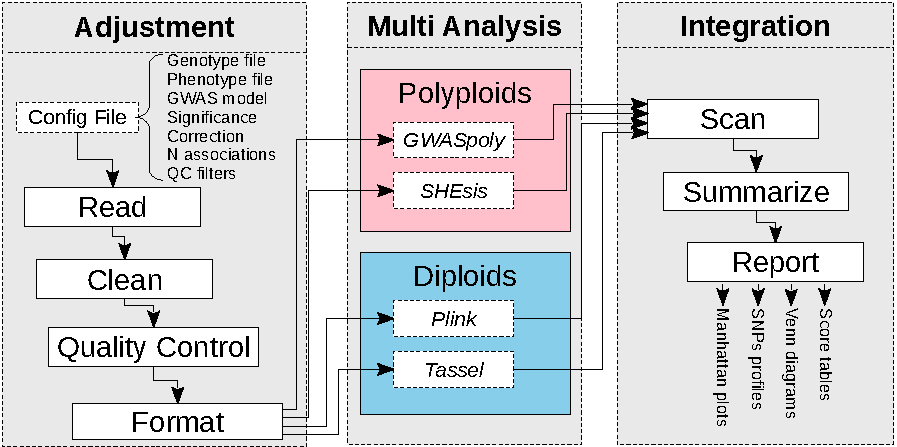
\includegraphics[scale=0.55]{images/multi-gwas-flowchart-horizontal-stages-config}
\par\end{centering}
\caption{Flowchart of the central steps in the MultiGWAS tool. The analysis
is carried out by in three stages: adjustment, multi analysis, and
integration. In the first stage, inputs are read from a configuration
file (see below) and the genotype and phenotype are cleaned and filtered
using the quality control (QC) filters. In the second stage, the new
filtered genotype/phenotype are formated for each GWAS tool which
are executed in parallel. In the last stage, the output files generated
from each tool are scanned, and their results are summarized and reported
through score tables, Venn diagrams, SNP profiles, and Manhattan plots.
The configuration file includes: the genotype/phenotype filenames,
genome-wide significance threshold, multiple testing correction method,
GWAS model, number of associations to be reported, and TRUE or FALSE
whether to use QC filters or not. The QC filters are: minor allele
frequency, individual missing rate, SNP missing rate, Hardy-Weinberg
threshold. \label{fig:Flowchar}}
\end{figure}

\begin{figure}
\begin{centering}
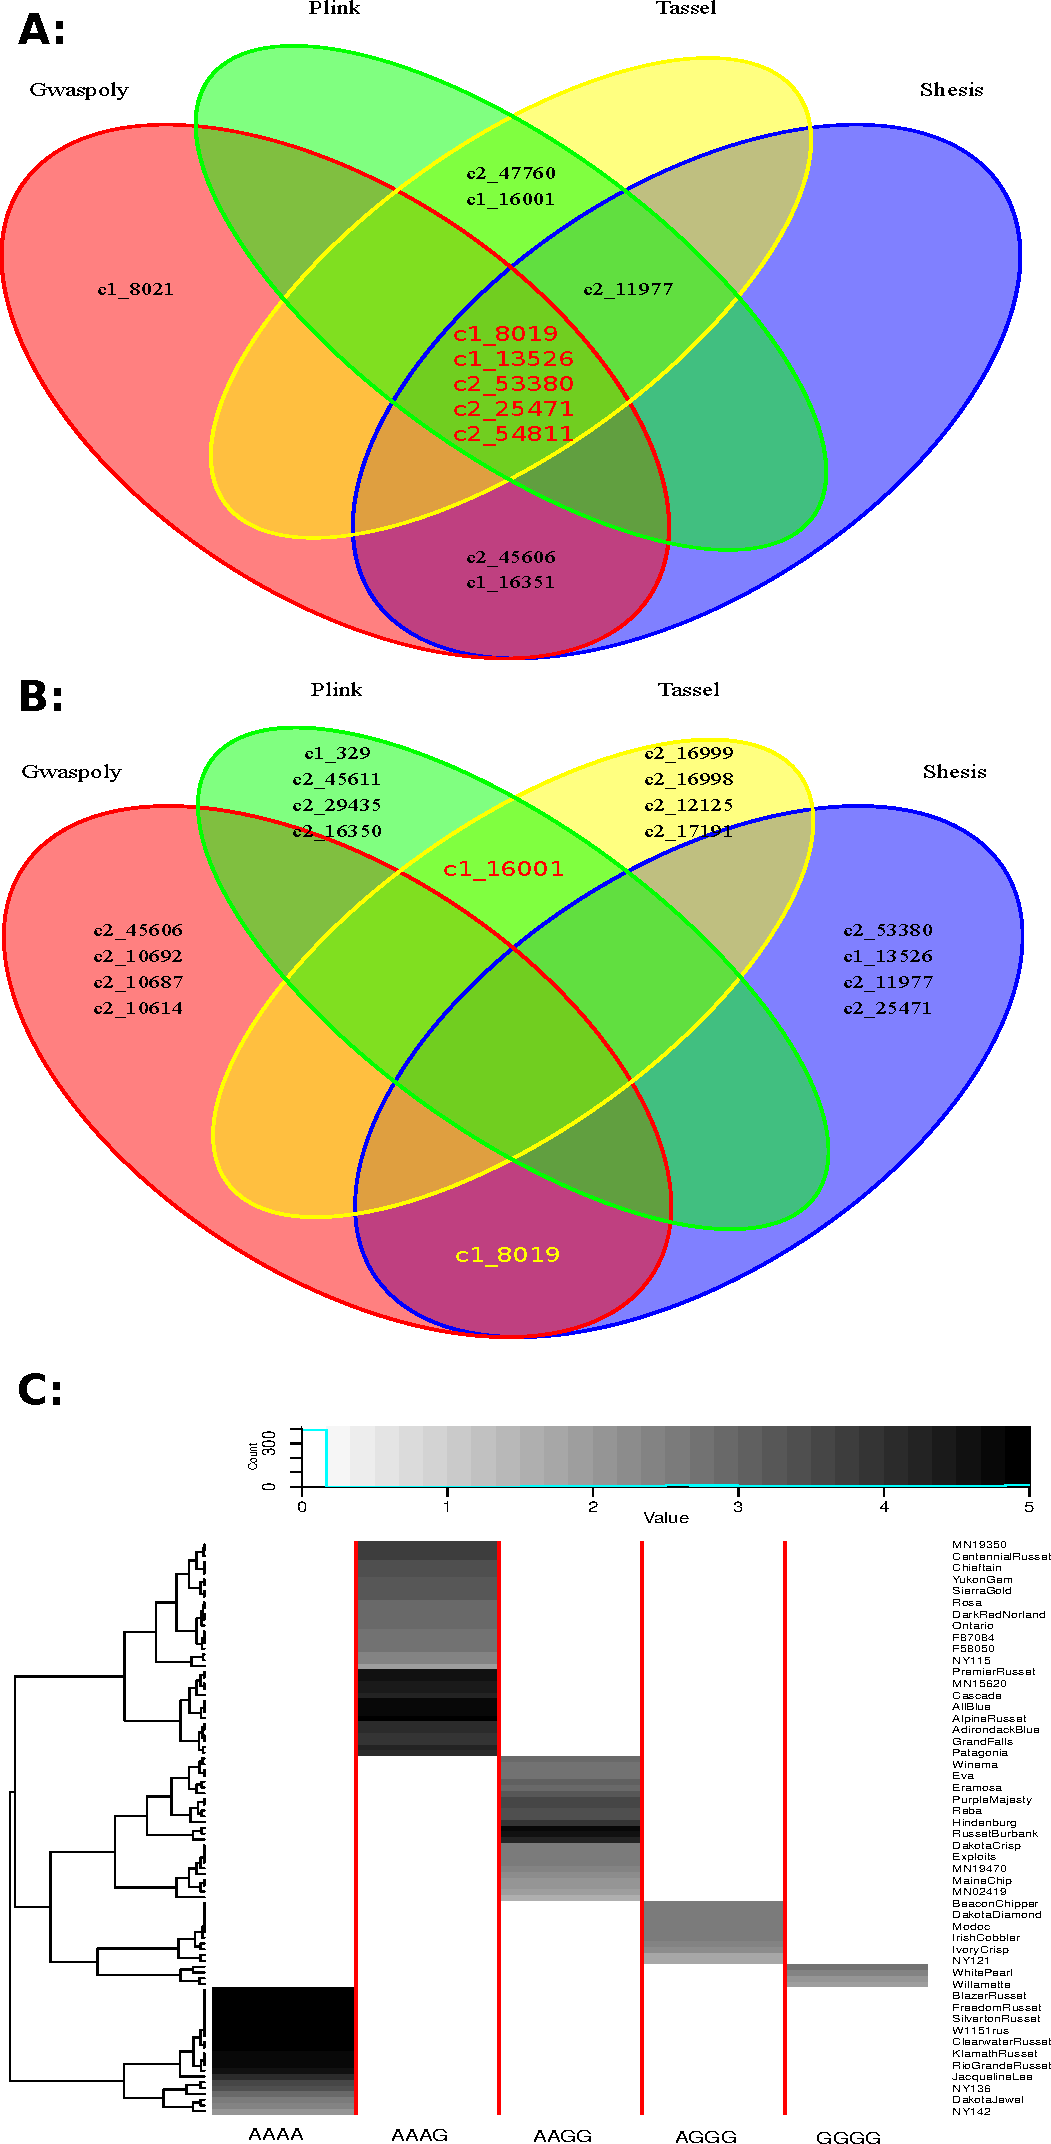
\includegraphics[bb=0bp 0bp 505bp 1029bp,scale=0.43]{images/out-Gwaspoly-Both-Naive-Bonf-Sign-Structure-Bonf-Best5-Profile}
\par\end{centering}
\caption{Venn diagrams and SNP profile generated by the MultiGWAS tool for
the SolCAP potato panel. A: GWAS with Naive model in which the four
software found the same set of five markers (center area, red text).
B, GWAS with Full model in which the two diploid software found one
common marker (upper-central area, red text), but the other two polyploid
tools found a different common marker (lower-central area, yellow
text). In both cases, other marker were found either by two or by
one software. \label{fig:Cases}}
\end{figure}


\section{Introduction}

Genome-wide association studies (GWAS) allows to analyze genomic data
to identify the set of variants across different individuals of a
species that are associated with a phenotypic characteristic of research
interest. Due to the advances in the next-gen sequencing technology,
GWAS analysis are currently more frequently used in non-model species
as plants which include polyploid crops, that are important for agriculture
and the food security of different developing countries. 

One of the main challenges in these GWAS analysis is to identify true
from false associations, which can be validated by replicating the
analysis using different tools. However, each tool has its own characteristics
with different user interfaces (GUI or command line based), genotype/phenotype
formats, models and algorithm assumptions, and different outputs,
all of which take great effort to consider and makes it difficult
for researches to do the replicatation.

The two most strong tools to perform GWAS across different organisms
are Plink \cite{Purcell2007} and Tassel \cite{Bradbury2007}. However,
both are limited to diploid species and to be used for polyploids,
the genomic data need to be ``diploidized'' \cite{Lindqvist2014,Shulz2016}.
Fortunately, in 2016 were published two software explicitly designed
for GWAS in polyploid species. They are the R package GWASpoly \cite{Rosyara2016}
and the SHEsis tool \cite{Shen2016}.

With these considerations in mind, we developed the MultiGWAS tool
that performs GWAS analyses by using four different GWAS software.
The tool deals with all matters of the GWAS process in the four software:
preprocessing genomic data using different quality control filters,
transforming it to particular tool formats, executing each GWAS software
in parallel, postprocessing outputs and creating reports. The reports
provides the user with tables and plots showing the significative
and best ranked markers, also the markers found by one tool and by
more than one tool, all of this with the objecive to help users to
decide in a more intuitively way the possible true or false associations.


\section{Methods and Implementation}

A flowchart of the main central steps involved in the three stages
of the MultiGWAS tool is outlined in figure \ref{fig:Flowchar}.


\subsection{Adjustment stage\label{subsec:Adjust}}

MultiGWAS takes as input a configuration file where the user specifies
the genomic data along with the parameters that will be used by the
four tools to perform their particular GWAS analysis (see figure \ref{fig:Flowchar}).
It starts by preprocessing the genomic data by selecting individuals
present in both genotype and phenotype, and excluding individuals
and SNPs that are likely to be of poor-quality. 

The allowed format for the marker data is the ''ACGT'' (e.g. AAAT,
... ,CCCG), suitable for the polyploid software GWASpoly and SHEsis,
but what is needed to ``diploidize'' for Plink and Tassel (e.g.
AT, ... ,CG). MultiGWAS does this by coding each marker in one of
two possible ways: all possible homozygous genotypes are coded with
two nucleotides (AAAA\textrightarrow AA, CCCC\textrightarrow CC, GGGG\textrightarrow GG,
TTTT\textrightarrow TT); and all possible heterozygous genotypes are
coded with the combination of their reference and alternate alleles
calculated from the tetraploid marker (e.g. AAAT\textrightarrow AT,
... ,CCCG\textrightarrow CG). After that, the new filtered genotype
and phenotype are transformed to the specific formats required for
each tool using different own functions from MultiGWAS. 


\subsection{Multi analysis stage}

The four tools are executed in parallel by MultiGWAS using for each
one a particular script parameterized with the transformed genotype/phenotype
and parameters set in the configuration file (see figure \ref{fig:Flowchar}).
One of these parameters is the type of statistical GWAS model to be
conducted, where MultiGWAS allows two of them: Full (Q+K) and Naive
\cite{Sharma2018}. The first with control for population structure
and individual relatedness; and the second without any of these controls.
Controlling of population structure is based on the principal components
(PCs) where each tool calculates the PCs and uses the top ten as covariates
in their GWAS analysis. Controlling of individual relatedness is based
on kinship matrices, where Tassel and GWASpoly make their own calculations,
but Plink and SHEsis calculate them externally by the king software
\cite{Manichaikul2010}.

 


\subsection{Integration stage}

The outputs resulting from the four tools are scanned and processed
to identify the SNPs with both: significant and best ranked associations.
This is done by correcting the reported \emph{p-values}, and calculating
their threshold value using the correction method and significance
level $\alpha$ set in configuration file. These values are calculated
taking into account only the number of valid genotype calls (nonmissing
genotype, phenotype, and covariates). All this information is summarized
to report them as tables and Venn diagrams for significative and best
ranked associations, SNPs profiles, and Manhattan plots.


\section{Results and Discussion}

Figure 2 presents two marker plots generated by MultiGWAS in the analysis
of the genomic data for the Solanaceae Coordinated Agricultural Project
(SolCAP) potato diversity panel, used to test the GWASpoly software
for polyploid species \cite{Rosyara2016}. In the first case (figure
\ref{fig:Cases}.A), it shows that the four software agreed on a large
set of common markers (text in red, figure \ref{fig:Cases}.A). It
can be explained as the statistical GWAS model used was Naive, without
any controls for population structure or individual relatedness. However,
two markers from this set, c1\_8019 and c2\_25471, were also reported
by Rosayra et al., the first as the most significative association,
and second as the second best ranked association. So, the four tools
agreed

In the second case (figure \ref{fig:Cases}.B), it shows that the
set of common markers found by the tools was reduced, which can be
explained as the statistical GWAS model used was Full, with controls
for population structure (10 PCs) and individual relatedness (kinship
matrix). Now, the two polyploid tools GWASpoly and SHEsis found the
common marker c1\_8019, as in the Naive GWAS, which help us to consider
whit more confidence that this marker is a true association. But,
the two diploid tools found a different common marker, the c1\_16001,
which was nof found in the first case (figure \ref{fig:Cases}.A)
and may be a false association. 

\bibliographystyle{natbib}
\bibliography{multiGWAS}

\end{document}
